\chapter{Hardware Characterisation}
\label{chap:hardware}
\chaptoc{}

% ########################################

\newpage
\section{Introduction}
\label{sec:hardware_intro}
\begin{colsection}

% ~~~~~~~~~~~~~~~~~~~~

\begin{colsection}

\rtxt{TODO}

\end{colsection}

% ~~~~~~~~~~~~~~~~~~~~
\subsection{Properties of a CCD}
\label{sec:CCDs}
\begin{colsection}

% ---------
\subsubsection{Sources of noise}

There are multiple sources of noise in images taken with CCD cameras \citep{CCDs}:

\begin{itemize}
    \item Shot noise derived from counting photo-electrons from the source object.
    \item Dark current noise, shot noise from thermally generated electrons within the sensor.
    \item Read-out noise from the camera electronics.
    \item Fixed-pattern noise from different sensitivities between pixels.
    \item Bias count, a fixed level of output for each pixel.
\end{itemize}

The shot noise ($\sigma_\text{O}$) comes from photons arriving at the sensor at different times. The photon arrival time is a Poisson distribution, and if the number of electrons counted is $N$, for large numbers of photons this tends towards a Gaussian distribution with mean $N$ and standard deviation $\sigma_O = \sqrt{N}$. When carrying out on-sky astronomical observations the source noise is typically divided into noise from the target object and noise from the background sky, but this is not relevant for the in-lab tests described in this section.

Dark current noise ($\sigma_\text{D}$) is due to electrons produced by thermal excitations, these are indistinguishable from photo-electrons and will increase with exposure time. As this is also a photon counting measurement it also follows a Poisson distribution, so the noise $\sigma_D = \sqrt{D}$ where $D$ is the dark current per pixel. Cooling the cameras will reduce the thermal excitations and therefore reduce the dark current.

Read-out noise ($\sigma_\text{RO}$) depends on the speed data is read out from the CCD.\ The FLI MicroLine cameras read out at a fixed \SI{8}{\mega\hertz}, but other astronomical cameras have variable read-out speeds. As a property of the output electronics the read-out noise is independent of signal or the exposure time used, and therefore it can be represented by a constant value, $\sigma_R = R$, measured in electrons. The MicroLine cameras have two channels with independent readouts, so each will have an independent read-out noise.

Fixed-pattern noise ($\sigma_\text{FP}$) is due to the small differences in size and response between pixels. It it increases linearly with the electron count, including both source and dark electrons (the fixed-pattern noise can be further broken down into the \gls{prnu} and \gls{dsnu}, but we will consider it as a single noise source). Including both these effects the fixed-pattern noise can be parametrised as $\sigma_\text{FP} = k_\text{FP}(N+D)$ where $k_\text{FP}$ is a dimensionless constant of proportionality describing the fixed-pattern noise as a percentage of the full-well capacity. Scientific CCD cameras typically have very small non-uniformities between pixels, so $k_\text{FP}$ is usually $<1\%$, but this noise source can dominate when the signal count is high. It can however be removed by flat fielding, so the fixed-pattern noise is often not considered in astronomical contexts.

Finally, the bias level is a fixed output of counts from each pixel, and is entirely independent of the input signal. It is therefore the easiest noise source to account for, as once a master bias frame has been constructed it can simply be subtracted from each frame. The MicroLine cameras also include an overscan region described previously, which gives an independent measurement of the bias level.

The noises described above (aside from the bias) are all independent Gaussian random variables, and therefore are added in quadrature to get the total noise per pixel

\begin{equation}
    \begin{split}
        \sigma_\text{Total}^2 & = \sigma_\text{O}^2 +
                                  \sigma_\text{DC}^2 +
                                  \sigma_\text{RO}^2 +
                                  \sigma_\text{FP}^2 \\
                              & = N + D + R^2 + k_\text{FP}^2{(N+D)}^2.
    \end{split}
    \label{eq:noise}
\end{equation}

\end{colsection}

% ~~~~~~~~~~~~~~~~~~~~

\end{colsection}

% ########################################

\newpage
\section{Detector properties}
\label{sec:detectors}
\begin{colsection}

% ~~~~~~~~~~~~~~~~~~~~

\begin{colsection}

CCD cameras have a variety of characteristic parameters as described above, including sources of noise, and analysing the in laboratory conditions is important to fully profile them before they are used to take scientific images. The camera manufacturer \glsfirst{fli} and detector manufacturer ON Semiconductor both produce specification sheets advertising expected parameters\footnote{\url{http://www.flicamera.com/spec_sheets/ML50100.pdf}}\textsuperscript{,}\footnote{\href{http://www.onsemi.com/pub/Collateral/KAF-50100-D.PDF}{\texttt{http://www.onsemi.com/pub/Collateral/KAF-50100-D.pdf}}}, and FLI carried out a limited series of tests on the cameras before selling them. Carrying out our own tests ensures that the cameras meet the specifications, and also allows independent measurements of the key parameters.

\end{colsection}

% ~~~~~~~~~~~~~~~~~~~~
\subsection{In-lab tests}
\label{sec:camera_tests}
\begin{colsection}

The initial deployment of GOTO was delayed for several months, due to delays on-site at the observatory on La Palma and manufacturing the unit telescopes. The cameras however had already been purchased from FLI, and the delay gave time to test them in the lab in Sheffield. The second set of cameras were also purchased long before the second four unit telescopes were built, these were also bought to Sheffield so the same tests could be repeated.

A list of the nine FLI cameras bought for GOTO is given in \aref{tab:cameras}. Each camera is given a name (Camera 1, Camera 2 etc.) based on the order of their serial numbers. These do not match which GOTO unit telescope they were assigned to, and the cameras on La Palma are sometimes swapped around to allow for repairs.

The first set of four cameras arrived in Warwick in February 2016, and one (Camera 2) was bought to Sheffield in March with a collection of other hardware. The other three were delivered in May and Camera 2 was returned to Warwick, these three were returned in June. The second set cameras were delivered to Warwick in April 2018: four for the next four unit telescopes as well as a spare. The second four cameras (5--8) were brought to Sheffield in May, with Warwick keeping the spare for their own use, these were returned in June.

\begin{table}[t]
    \begin{center}
        \begin{tabular}{cccc} %chktex 44
            Name     & Serial number & Set & Tested \\
            \midrule
            Camera 1 & ML0010316     &   1 & May---June 2016  \\
            Camera 2 & ML0330316     &   1 & March---May 2016 \\
            Camera 3 & ML0420516     &   1 & May---June 2016  \\
            Camera 4 & ML0430516     &   1 & May---June 2016  \\
            Camera 5 & ML5644917     &   2 & May---June 2018  \\
            Camera 6 & ML6054917     &   2 & May---June 2018  \\
            Camera 7 & ML6094917     &   2 & May---June 2018  \\
            Camera 8 & ML6304917     &   2 & May---June 2018  \\
            Camera 9 & ML6314917     &   2 & N/A              \\
        \end{tabular}
    \end{center}
    \caption[List of GOTO cameras]{
        A list of the 9 GOTO cameras, with assigned names, serial numbers and when the tests were carried out.
    }\label{tab:cameras}
\end{table}

The characterisation tests consisted of taking a series of calibration frames with each camera. Three types of images were needed:

\begin{itemize}
    \item Zero-second dark exposures, to construct bias frames (see \aref{sec:bias}).
    \item Long (30 minute) dark exposures at different temperatures, to measure the dark current (see \aref{sec:dc}).
    \item Flat illuminated frames at different exposure times, to construct photon transfer curves (see \aref{sec:ptc}) and measure linearity (see \aref{sec:lin}).
\end{itemize}

The cameras were tested using two different test setups. \aref{fig:dark_photo} shows the setup for taking dark frames: the cameras are face down and covered. The long dark exposures were taken overnight to as much as possible reduce any excess light reaching the detectors. The flat frames were harder to take. A LCD monitor showing a dark screen was used, with sheets of paper between the camera and the monitor to reduce the illumination. This is shown in \aref{fig:flat_photo}.

\begin{figure}[p]
    \begin{center}
        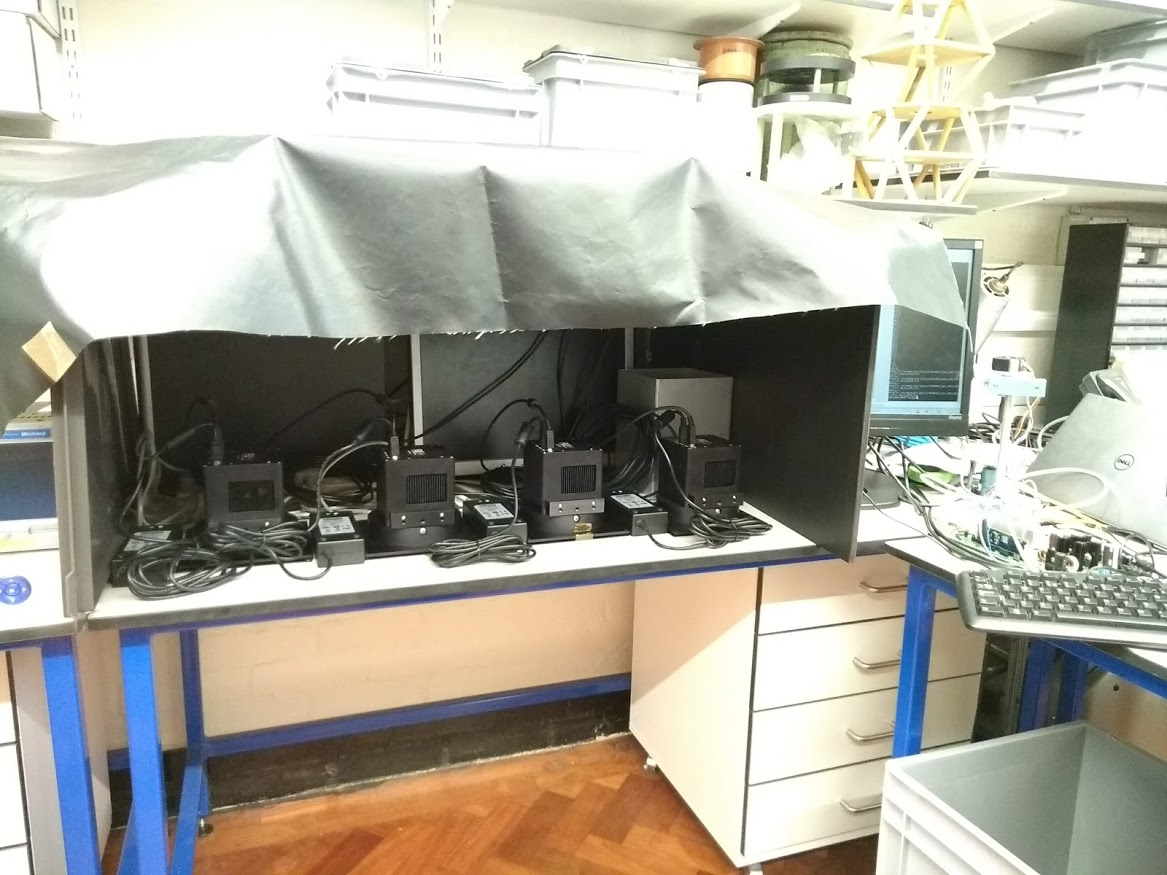
\includegraphics[width=0.75\textwidth]{images/dark_photo.jpg}
    \end{center}
    \caption[The dark frame test setup]{
        A photo of the dark frame test setup in the lab in Sheffield. Dark frames were taken at night with the cover down and the ambient light minimised as much as possible.
    }\label{fig:dark_photo}
\end{figure}

\begin{figure}[p]
    \begin{center}
        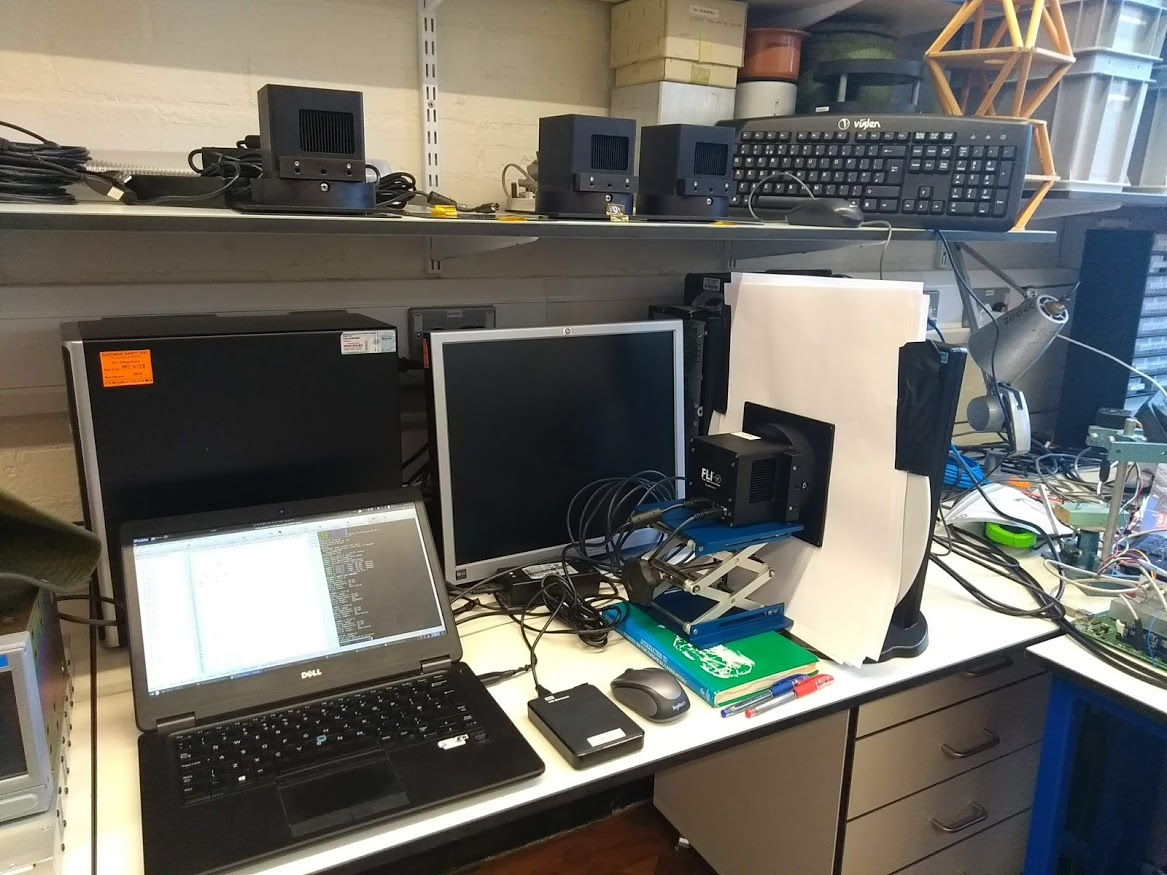
\includegraphics[width=0.75\textwidth]{images/flat_photo.jpg}
    \end{center}
    \caption[The flat frame test setup]{
        A photo of the flat frame test setup. In the absence of a flat illuminated screen a spare computer monitor was used, with sheets of paper placed in front of the camera to reduce the illumination. The cover shown in \aref{fig:dark_photo} was also placed over the setup.
    }\label{fig:flat_photo}
\end{figure}

\clearpage

\end{colsection}

% ~~~~~~~~~~~~~~~~~~~~
\subsection{Sensor layout}
\label{sec:sensors}
\begin{colsection}

The MicroLine ML50100 cameras used by GOTO are contain a KAF-50100 CCD sensor manufactured for FLI by ON Semiconductor\footnote{\url{http://www.onsemi.com/}}. The sensor consists of a 50-megapixel CCD with $\SI{6}{\micro\metre} \times \SI{6}{\micro\metre}$ square pixels. The sensors in the GOTO cameras have two channels each with an independent output, and read out at \SI{8}{\mega\hertz} (variations with four outputs and different readout speeds are also available).

The layout of the sensor is shown in \aref{fig:chip}, adapted from the ON Semiconductor sensor specification sheet. The physical sensor includes $8304 \times 6220$ pixels, while the central region available for data collection has an area of $8176 \times 6132$ pixels. When taking data in full-frame mode the camera outputs an $8304 \times 6220$ array. Surrounding the active area on each edge are 16 \emph{active buffer pixels}, which are light-sensitive but not considered part of the primary region. Around the edge of the active area is a border of light-shielded \emph{dark reference pixels}: 29 dark rows at the start, 26 rows at the end and 28 columns on the sides leading each row. These pixels do not respond to light and therefore can be used as a dark reference. At the beginning and end of each row there is also a test column with 4 blank columns either side, as well as a test row at the end of each frame; these are used to test charge transfer efficiency during the manufacturing process. Finally at the start of each row the register reads out one text pixel, used in the readout process, followed by 10 \emph{dummy pixels} which do not correspond to physical pixels on the sensor. These dummy pixels form an overscan region which can be used to measure the bias level.

A sample frame from Camera 2 is shown in \aref{fig:frame} at high contrast. The extra regions around the frame are visible, including the dark reference and overscan regions.

\begin{figure}[p]
    \begin{center}
        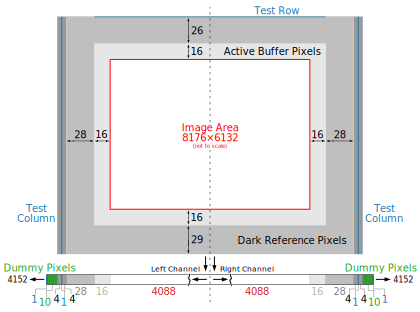
\includegraphics[width=0.85\textwidth]{images/chip}
    \end{center}
    \caption[The layout of the CCD chips in the MicroLine cameras used by GOTO]{
        The layout of the CCD chips in the MicroLine cameras used by GOTO.\@ The central image area is not shown to scale, but the surrounding rows and columns are all in proportion.
    }\label{fig:chip}
\end{figure}

\begin{figure}[p]
    \begin{center}
        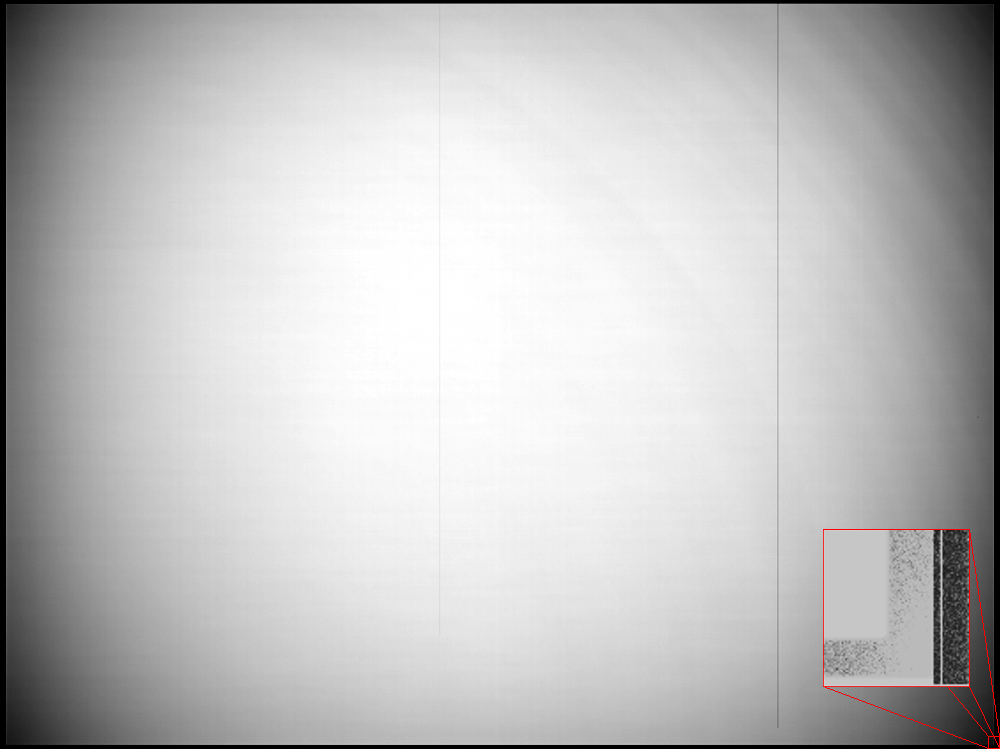
\includegraphics[width=0.7\textwidth]{images/sample.png}
    \end{center}
    \caption[A sample bright frame from one of the MicroLine cameras]{
        A sample bright frame from one of the MicroLine cameras. The highlighted area in the corner shows some of the features described in \aref{fig:chip}.
    }\label{fig:frame}
\end{figure}

\clearpage

\end{colsection}

% ~~~~~~~~~~~~~~~~~~~~
\newpage
\subsection{Bias}
\label{sec:bias}
\begin{colsection}

The bias level is a fixed offset in counts for each pixel. Setting a reasonable bias level in a CCD is important in order to ensure counts are never recorded as negative due to random noise. In general the bias level of each pixel is considered a fixed value, although it can change over time due to degradation of the pixel electronics. Bias should therefore still be measured regularly, as any change might indicate a problem with the detector.

Pixel bias levels can be measured by taking a dark, zero-second exposure time image. This image will not include any electrons from a source, so the shot noise is zero, and as the dark current is proportional to the exposure time this will also be minimised. The image will however still include random read-out noise, so to account for this multiple images are taken and then averaged to produce a master bias frame.

For each of the eight cameras 50 bias images were taken, these were combined to form a master bias frame by taking the median value in each pixel (to account for superfluous counts due to cosmic rays). The mean count in a 2000$\times$2000 pixel region in the centre of each of the two camera channels was measured, using a one-sigma clip to exclude any defect pixels (see \aref{sec:defects}). These values are given in \aref{tab:bias}.

The measured biases are all around the same level, 970--1010 counts, as would be expected. They also have a uniform standard deviation of approximately 0.3--0.4\% of the signal, which will come from the fixed-pattern noise (see \aref{sec:ptc}).

\begin{table}[t]
    \begin{center}
        \begin{tabular}{c|rr} %chktex 44
             & \multicolumn{2}{c}{Bias} \\
             & \multicolumn{2}{c}{(ADU)} \\
             & \multicolumn{1}{c}{L} & \multicolumn{1}{c}{R} \\
            \midrule
            Camera 1 & $971\pm4$ & $969\pm4$ \\
            Camera 2 & $989\pm3$ & $983\pm3$ \\
            Camera 3 & $1004\pm3$ & $991\pm3$ \\
            Camera 4 & $974\pm3$ & $1008\pm4$ \\
        \end{tabular}
        \hspace{0.5cm}
        \begin{tabular}{c|rr} %chktex 44
             & \multicolumn{2}{c}{Bias} \\
             & \multicolumn{2}{c}{(ADU)} \\
             & \multicolumn{1}{c}{L} & \multicolumn{1}{c}{R} \\
            \midrule
            Camera 5 & $994\pm3$ & $986\pm3$ \\
            Camera 6 & $984\pm3$ & $991\pm3$ \\
            Camera 7 & $992\pm3$ & $981\pm3$ \\
            Camera 8 & $1008\pm3$ & $1012\pm3$ \\
        \end{tabular}
    \end{center}
    \caption[Bias values]{
        Bias values for each camera.
    }\label{tab:bias}
\end{table}

\end{colsection}

% ~~~~~~~~~~~~~~~~~~~~
\newpage
\subsection{Gain, read-out noise and fixed-pattern noise}
\label{sec:ptc}
\begin{colsection}

The gain, read-out and fixed-pattern noise of a CCD camera can be measured using the \gls{ptc} method \citep{CCDs, PTC}. To construct a photon transfer curve a series of bright exposures of a flat light source were taken with varying exposure times. For these images the dark current noise is negligible, so once the images has the bias level subtracted the total number of electrons in each pixel, $N_\text{Total}$, will include a number of photo-electrons from the source $N$ plus extra electrons from the readout electronics $R$:

\begin{equation}
    N_\text{Total} = N + R.
    \label{eq:total_count}
\end{equation}

The noise per pixel, excluding dark current, is given by \aref{eq:noise} as

\begin{equation}
    \begin{split}
        \sigma_\text{Total}^2 & = N + R^2 + k_\text{FP}^2 N^2 \\
                              & = N_\text{Total} - R + R^2 + k_\text{FP}^2{(N_\text{Total} - R)}^2.
    \end{split}
    \label{eq:ptc_noise1}
\end{equation}

The counts and total noise here are all in electrons (\elec), however the output of the camera analog-to-digital converter is a digital signal, $S$, measured in \gls{adu}. This signal is linearly related to the actual number of electrons detected $N_\text{Total}$ through the gain $g$, in \elec/ADU, as

\begin{equation}
    N_\text{Total} = g S.
    \label{eq:gain}
\end{equation}

The gain is an important parameter of a CCD detector, and can be set to best utilise the dynamic range of the detector. The KAF-50100 detectors have a specification full well capacity of 40,300 electrons before they saturate, and the cameras have a 16-bit readout (meaning the signal from each pixel can vary from 0 to 65535 ($2^{16}$) ADU). Therefore if the gain was set to $1$ \elec/ADU a saturated pixel would produce a signal of 40300 ADU, which is only using two-thirds of the dynamic range. The ideal gain to utilise the full well capacity for these cameras would therefore be $0.62$ \elec/ADU.\@ However, a high gain introduces a quantisation error due to the random electrons produced by the read-out noise. Setting the gain therefore is a balance between these two effects.

Since \aref{eq:gain} shows the signal $S$ is directly proportional to the number of electrons $N$, their errors are also directly proportional with the same constant. Therefore the noise in the signal, $\sigma_S$, is related to the noise in the total electron count as

\begin{equation}
    \sigma_\text{Total} = g \sigma_S.
    \label{eq:noise_gain}
\end{equation}

Converting the total electron count and noise in \aref{eq:ptc_noise1} into ADU results in

\begin{equation}
    g^2\sigma_S^2 = gS - R + R^2 + k_\text{FP}^2 {(gS - R)}^2,
    \label{eq:ptc_noise2}
\end{equation}

and rearranging this gives the final photon transfer curve equation

\begin{equation}
    \sigma_S^2 = \frac{R^2(1-k_\text{FP}^2) - R}{g^2} + \frac{1}{g}S + k_\text{FP}^2 S^2.
    \label{eq:ptc}
\end{equation}

This is a quadratic equation in $S$ which relates the measured total signal $S$ to the variance in the signal $\sigma_S^2$, where $S$ and $\sigma_S$ are in ADU, read-out noise $R$ is still in \elec, gain $g$ is in \elec/ADU and the fixed-pattern noise parameter $k_\text{FP}$ is dimensionless. Since $k_\text{FP}$ is expected to be a very small fraction, typically less than 1\%, the $(1-k_\text{FP}^2)$ factor is often ignored. As well the constant is often further simplified to just $R^2/g^2$, which could be considered as $R_S^2$ where $R_S$ is measured in ADU.\@ For this test the full equation was used when fitting to the data.

A photon transfer curve is a log-log plot of a signal value against the noise in the signal, here represented by $S$ and standard deviation $\sigma_S$ (the square root of the variance). By fitting \aref{eq:ptc} to this plot values for the gain, read-out noise and fixed-pattern noise can be determined. The key features of a photon transfer curve are common for all CCDs, and are shown in cartoon form in \aref{fig:ptc_cartoon}.

\newpage

\begin{figure}[t]
    \begin{center}
        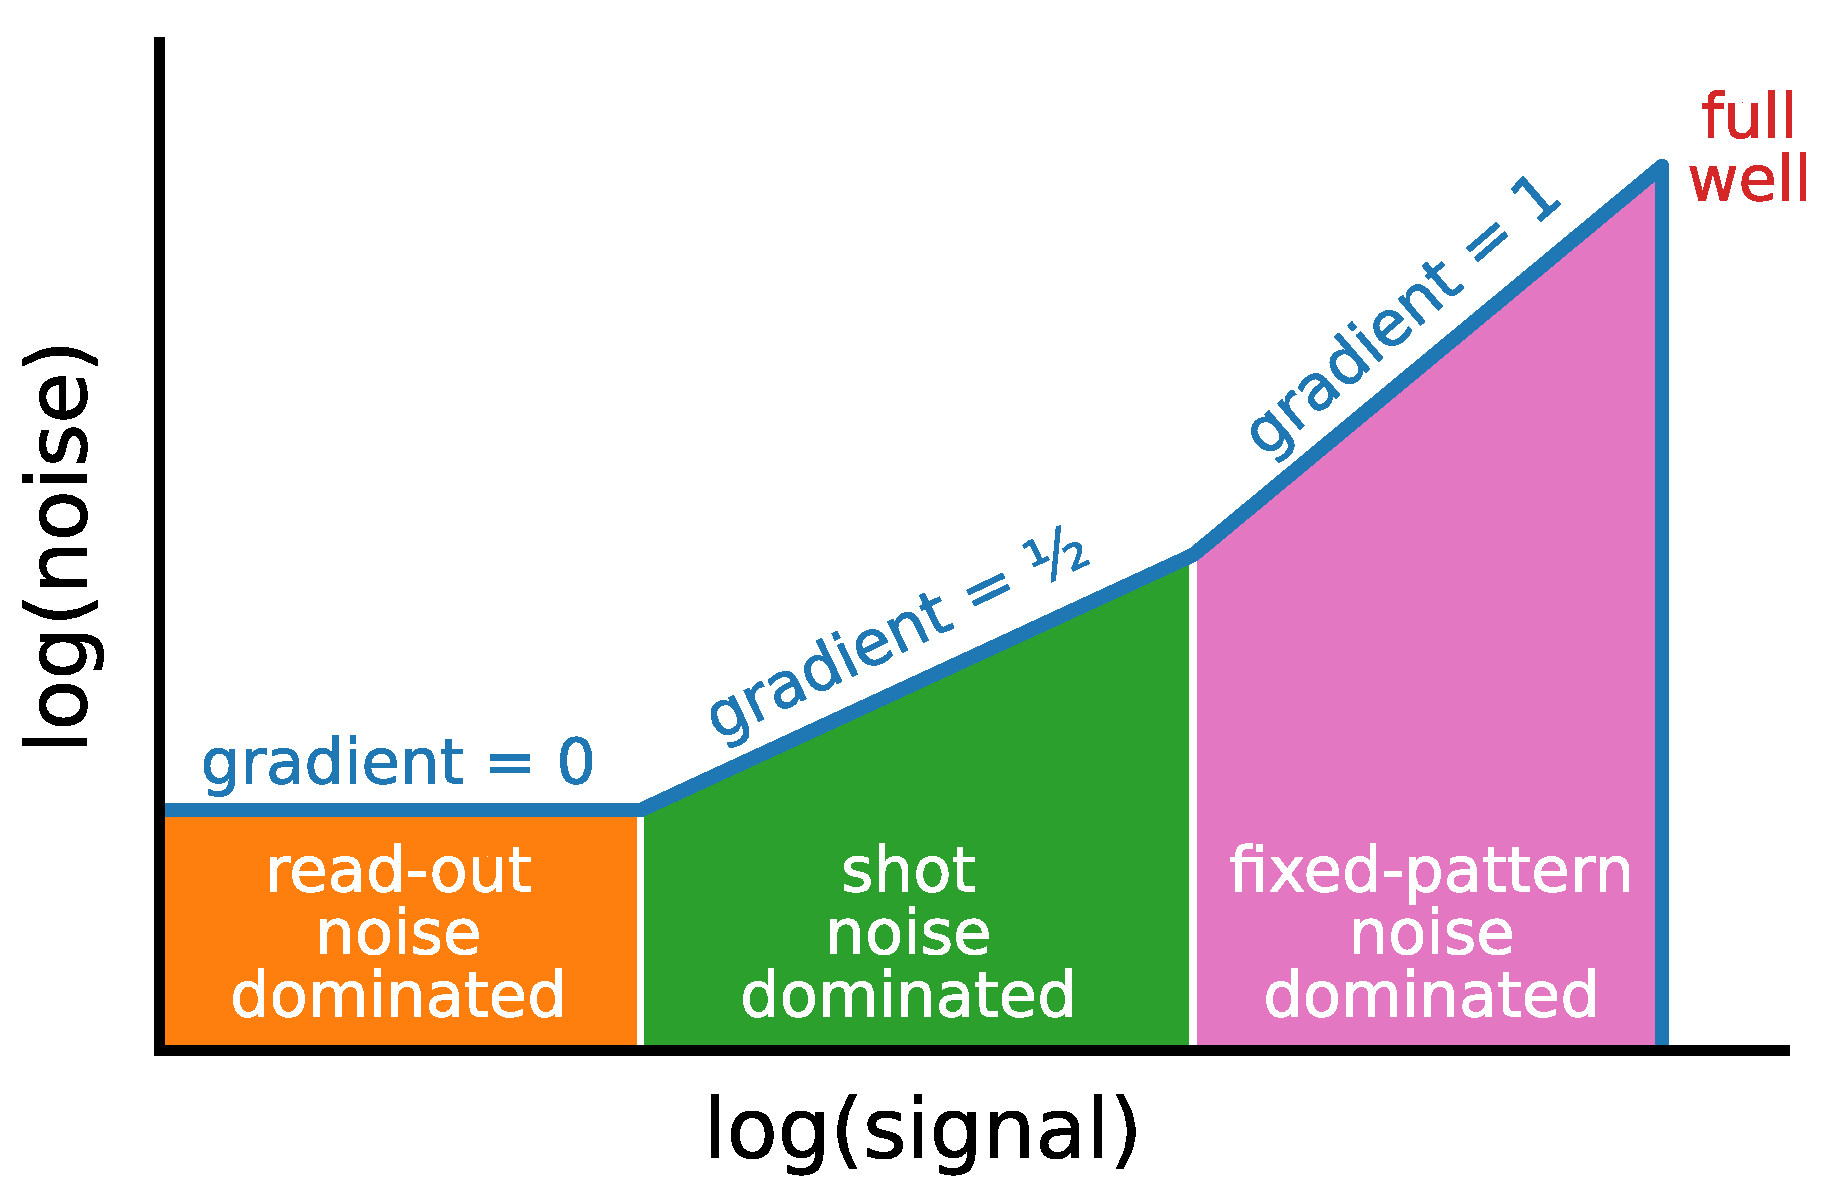
\includegraphics[width=0.65\textwidth]{images/ptc.pdf}
    \end{center}
    \caption[Key features of the photon transfer curve]{
        The key features of a photon transfer curve, adapted from Figure 2.2 of \citet{CCDs}.
    }\label{fig:ptc_cartoon}
\end{figure}

There are three visible noise regimes in the photon transfer curve. The first is when the signal is zero. For small $S$ in \aref{eq:ptc} the noise is constant, and as there is no signal the overall noise is limited by the detector noise. This will include both the read-out noise and the dark current, but as these are very short exposure times (less than 1 second) the dark current is completely negligible and the read-out noise dominates. At higher signals the noise is dominated by the shot noise. As this is proportional to the square root of the signal this region has a gradient of 1/2 when plotted on the log-log axis, and when $\sigma_S$ is zero the signal will equal the gain (i.e.\ the value of the gain is where the linear fit crosses the x-axis). As the signal increases further the fixed-pattern noise begins to dominate over the shot noise, as it is proportional to the signal this produces a gradient of 1 in the \gls{ptc}. Finally the pixel will reach its full well value and saturate, so the noise drops to zero.

As it is impossible to know the exact number of incoming photons on each pixel, it is not possible to determine the signal and noise values for a given pixel. Instead the PTC is constructed by selecting a region of pixels and plotting the mean signal value against the standard deviation. Repeated for several regions across the image this gives a reasonable approximation of the average noise in each pixel.

\newpage

\begin{table}[t]
    \begin{center}
        \begin{tabular}{l|cc|cc|cc} %chktex 44
             &
            \multicolumn{2}{c|}{Gain} &
            \multicolumn{2}{c|}{RO noise} &
            \multicolumn{2}{c}{FP noise} \\
            &
            \multicolumn{2}{c|}{(\elec/ADU)} &
            \multicolumn{2}{c|}{(\elec)} &
            \multicolumn{2}{c}{(\%)} \\
             & L & R & L & R & L & R \\
            \midrule
            Camera 1 & 0.53 & 0.53 & 12.9 & 12.6 & 0.46 & 0.45 \\
            Camera 2 & 0.53 & 0.53 & 12.4 & 12.2 & 0.44 & 0.46 \\
            Camera 3 & 0.57 & 0.57 & 13.1 & 12.3 & 0.45 & 0.42 \\
            Camera 4 & 0.57 & 0.58 & 14.0 & 14.5 & 0.41 & 0.43 \\
            Camera 5 & 0.62 & 0.63 & 12.8 & 13.3 & 0.40 & 0.40 \\
            Camera 6 & 0.63 & 0.62 & 12.4 & 13.1 & 0.40 & 0.40 \\
            Camera 7 & 0.62 & 0.62 & 13.6 & 13.1 & 0.41 & 0.39 \\
            Camera 8 & 0.62 & 0.62 & 14.8 & 12.8 & 0.41 & 0.39 \\
        \end{tabular}
    \end{center}
    \caption[Gain, read-out noise and fixed-pattern noise values]{
        Gain, read-out noise and fixed-pattern noise values found by fitting photon transfer curves for each camera.
    }\label{tab:ptc}
\end{table}

\glspl{ptc} were constructed for all eight cameras, by taking flat images of varying exposure times. Twelve 50$\times$50 pixel regions were selected across the field, and the mean and standard deviation of the pixel values were plotted to form the \gls{ptc}. These are shown in \aref{fig:ptcs}. The curves were fitted to \aref{eq:ptc}, and the resulting values for the gain ($g$), read-out noise ($R$) and fixed-pattern noise ($k_\text{FP}$) are given in \aref{tab:ptc}.

As expected, the gain values are all around 0.6 \elec/ADU, and would have been set as such to maximise the dynamic range. There is a clear difference in gain levels between the first set of cameras (1--4) and the second set (5--8), which is most likely due to changes made by FLI over the two years between their manufacture.

The read-out noise values match the FLI specifications which advertises a typical system noise of 12 \elec{} when reading out at \SI{8}{\mega\hertz}. The two channels on each camera are independent and therefore there is no correlation in read-out noise, unlike the gain which is always approximately the same in each amplifier.

Finally, as expected the fixed-pattern noise is a low fraction of the signal. It notably decreases from $\sim$0.45\% to $\sim$0.40\%; if this is related to improved chip manufacturing this may be related to the change in gain in the later cameras. However, this test only includes a small sample of the 50 million pixels on each chip and so may not be a perfect measure of the overall photo response non-uniformity. The values for the fixed-pattern noise also match the standard deviations measured in the master biases in \aref{sec:bias}.

\begin{figure}[p]
    \begin{center}
        \begin{minipage}[t]{0.49\textwidth}\vspace{10pt}
            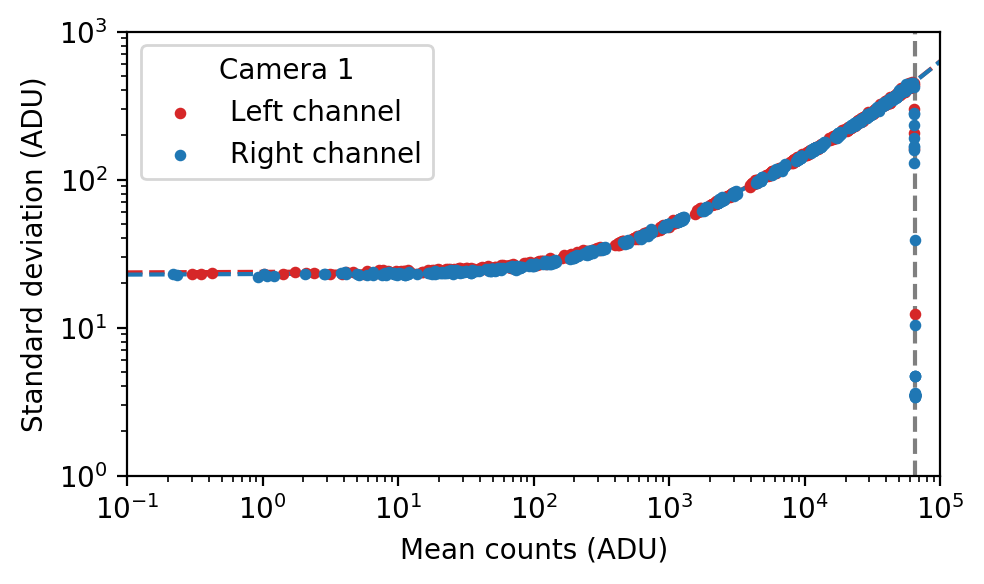
\includegraphics[width=\linewidth]{images/detectors/ptc_1.png}
        \end{minipage}
        \begin{minipage}[t]{0.49\textwidth}\vspace{10pt}
            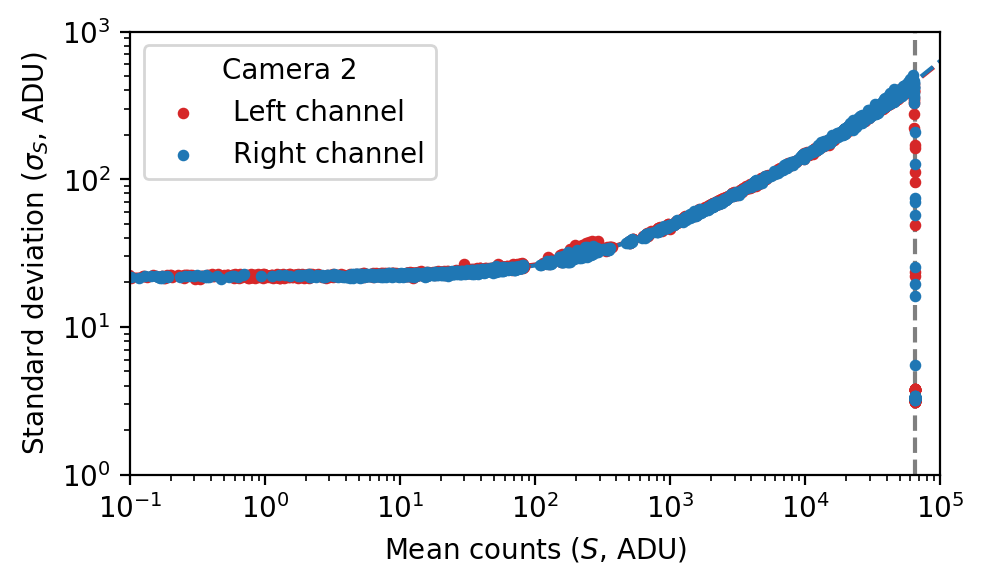
\includegraphics[width=\linewidth]{images/detectors/ptc_2.png}
        \end{minipage}

        \begin{minipage}[t]{0.49\textwidth}\vspace{10pt}
            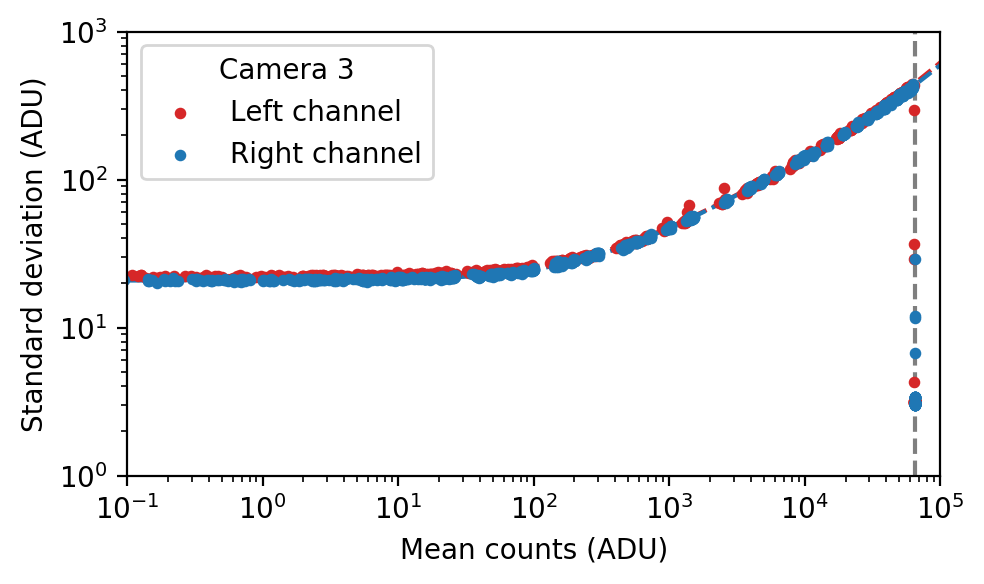
\includegraphics[width=\linewidth]{images/detectors/ptc_3.png}
        \end{minipage}
        \begin{minipage}[t]{0.49\textwidth}\vspace{10pt}
            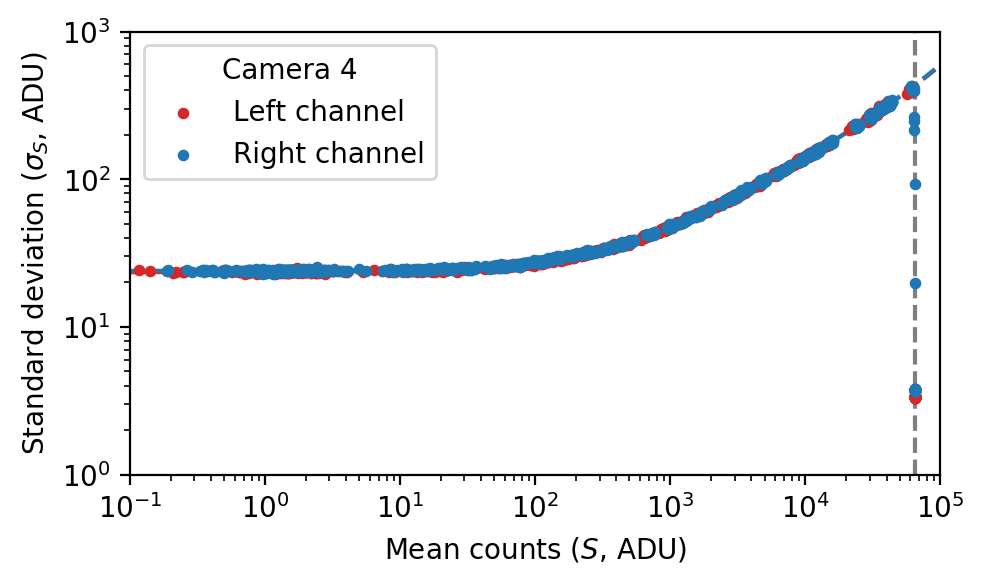
\includegraphics[width=\linewidth]{images/detectors/ptc_4.png}
        \end{minipage}

        \begin{minipage}[t]{0.49\textwidth}\vspace{10pt}
            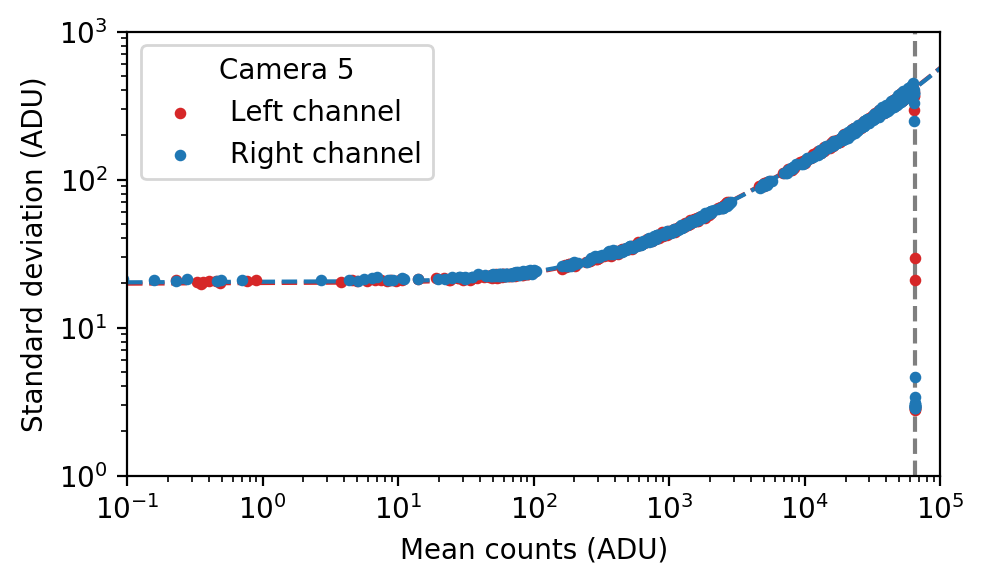
\includegraphics[width=\linewidth]{images/detectors/ptc_5.png}
        \end{minipage}
        \begin{minipage}[t]{0.49\textwidth}\vspace{10pt}
            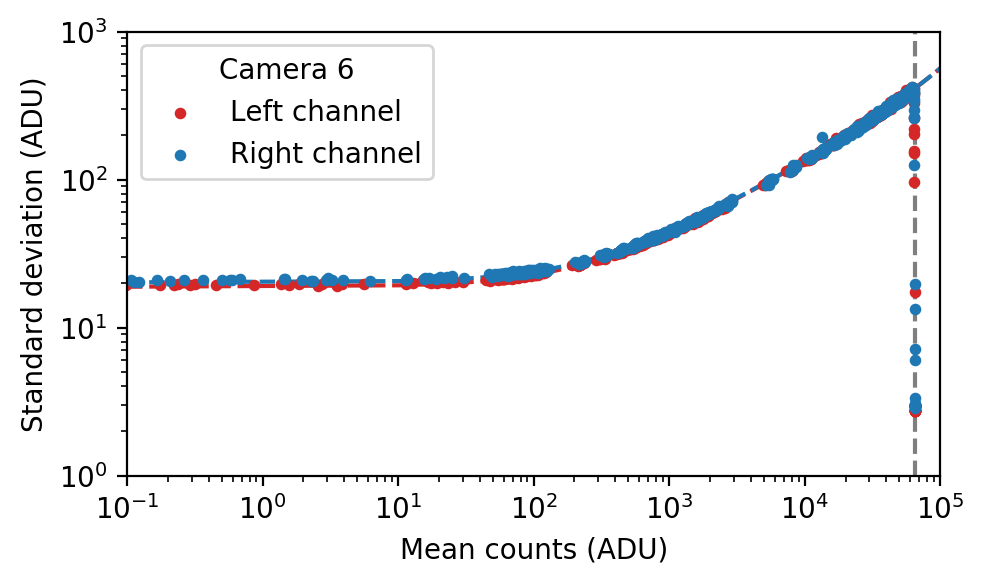
\includegraphics[width=\linewidth]{images/detectors/ptc_6.png}
        \end{minipage}

        \begin{minipage}[t]{0.49\textwidth}\vspace{10pt}
            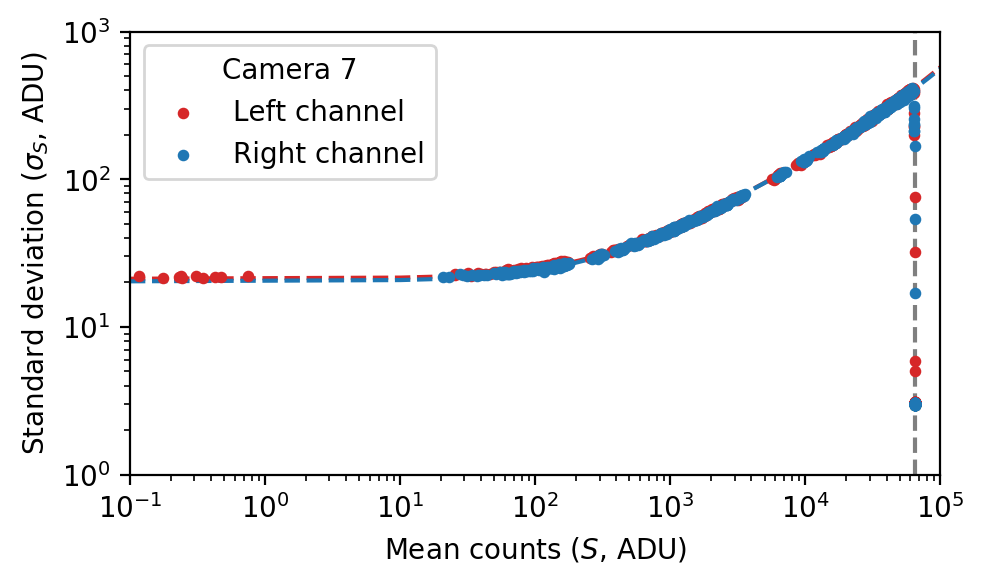
\includegraphics[width=\linewidth]{images/detectors/ptc_7.png}
        \end{minipage}
        \begin{minipage}[t]{0.49\textwidth}\vspace{10pt}
            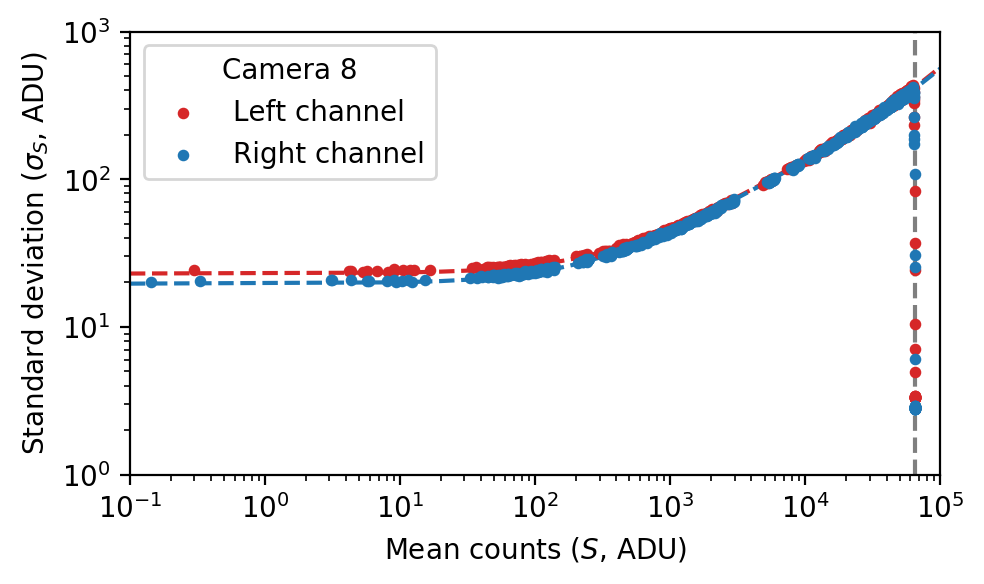
\includegraphics[width=\linewidth]{images/detectors/ptc_8.png}
        \end{minipage}
    \end{center}
    \caption[Photon transfer curve plots]{
        Photon transfer curve plots for each camera.
    }\label{fig:ptcs}
\end{figure}

\clearpage

\end{colsection}

% ~~~~~~~~~~~~~~~~~~~~
\newpage
\subsection{Dark current}
\label{sec:dc}
\begin{colsection}

Dark current is another source of noise in a CCD, produced by thermally excited electrons \citep{dark_current}. The dark current noise is therefore independent of the incoming signal or the exposure time, but increases as a function of temperature, $T$. Specifically the dark current increases at an exponential rate and so can be modelled in the form

\begin{equation}
    D(T) = Ae^{kT + C}
    \label{eq:dark_model}
\end{equation}

where $A$, $k$ and $C$ are constants. Dark current is usually defined as doubling after a fixed increase in temperature called the doubling temperature, $T_d$, so that if the dark current $D(T_0) = D_0$ then $D(T_0 + T_d) = 2D_0$. Redefining \aref{eq:dark_model} using these constants gives the equation for dark currant as

\begin{equation}
    D(T) = D_0 e^{\frac{\ln(2)}{T_d}(T + T_0)}.
    \label{eq:dc}
\end{equation}

The choice of $T_0$ is arbitrary, and is usually decided as a reasonable operating temperature by the CCD manufacturer. The FLI specifications give a value for the typical dark current at \SI{-25}{\celsius}, so that is the value of $T_0$ used in this test.

The MicroLine cameras have an in-built fan cooler which can reach \SI{40}{\celsius} below the ambient temperature. In order to find values for the dark current $D_0$ and doubling temperature $T_d$, a series of long (30 minute) dark exposures were taken with each camera at varying temperatures. The mean pixel count was then measured, and divided by 1800 to get the dark current in ADU/second. This value was plotted against temperature as shown in \aref{fig:dcs}. The points were fitted to \aref{eq:dc}, and the resulting values for the dark current and doubling temperature are given in \aref{tab:dc}.

\newpage

\begin{table}[t]
    \begin{center}
        \begin{tabular}{c|cc|cc|rr} %chktex 44
             &
            \multicolumn{4}{c|}{Dark current per pixel} &
            \multicolumn{2}{c}{Doubling} \\
             &
            \multicolumn{4}{c|}{at \SI{-25}{\celsius}} &
            \multicolumn{2}{c}{temperature} \\
             &
            \multicolumn{2}{c|}{(ADU/s)} &
            \multicolumn{2}{c|}{(e-/s)} &
            \multicolumn{2}{c}{(\SI{}{\celsius})} \\
             & L & R & L & R &
             \multicolumn{1}{c}{L} & \multicolumn{1}{c}{R} \\
            \midrule
            Camera 1 & 0.0022 & 0.0017 & 0.0012 & 0.0009 &  7.9 &  6.7 \\
            Camera 2 & 0.0030 & 0.0027 & 0.0016 & 0.0014 &  8.9 &  8.2 \\
            Camera 3 & 0.0034 & 0.0036 & 0.0019 & 0.0020 & 10.7 & 10.9 \\
            Camera 4 & 0.0026 & 0.0030 & 0.0015 & 0.0017 &  9.5 & 10.2 \\
            Camera 5 & 0.0015 & 0.0017 & 0.0009 & 0.0011 &  6.6 &  7.2 \\
            Camera 6 & 0.0020 & 0.0017 & 0.0013 & 0.0011 &  7.5 &  6.8 \\
            Camera 7 & 0.0017 & 0.0014 & 0.0011 & 0.0008 &  7.6 &  6.5 \\
            Camera 8 & 0.0019 & 0.0015 & 0.0012 & 0.0009 &  7.5 &  6.5 \\
        \end{tabular}
    \end{center}
    \caption[Dark current values]{
        Dark current values for each camera. The conversion from ADU/s to \elec/s used the gain values given in \aref{tab:ptc}.
    }\label{tab:dc}
\end{table}

The FLI MicroLine camera specification for dark current changed between the two test periods; initially it gave a typical per-pixel value of 0.002~\elec/s at \SI{-25}{\celsius}, but in between testing the two sets of cameras that was increased to 0.008~\elec/s. In order to convert the fitted value of dark current in ADU/s to e-/s the individual gain values found from the PTC were used, as listed in \aref{tab:ptc}. All the cameras were found to have a dark current well within the revised specification value, and all except Camera 3 are comfortably below the original 0.002~\elec/s specification.

The KAF-50100 specification includes a value for the dark current doubling temperature of \SI{5.7}{\celsius}, the measured values are all higher: between 6.5--\SI{11}{\celsius}. In practice the temperature dependence of the dark current is not important to GOTO, as the cameras are always cooled to \SI{-25}{\celsius} before images are taken and remain steady at that temperature throughout the night.

The dark current was also examined as a function of time since power on, as in some cameras there are a noticeable amount of free electrons left trapped in the lattice which take time to dissipate \citep{Liam}. No such trend was visible using the FLI cameras. Since the MicroLine cameras have the detector and cooler integrated into the same body there has to be some time spent waiting after power on for the camera to cool to the target temperature before any images could be taken, thus negating the effect.

\begin{figure}[p]
    \begin{center}
        \begin{minipage}[t]{0.49\textwidth}\vspace{10pt}
            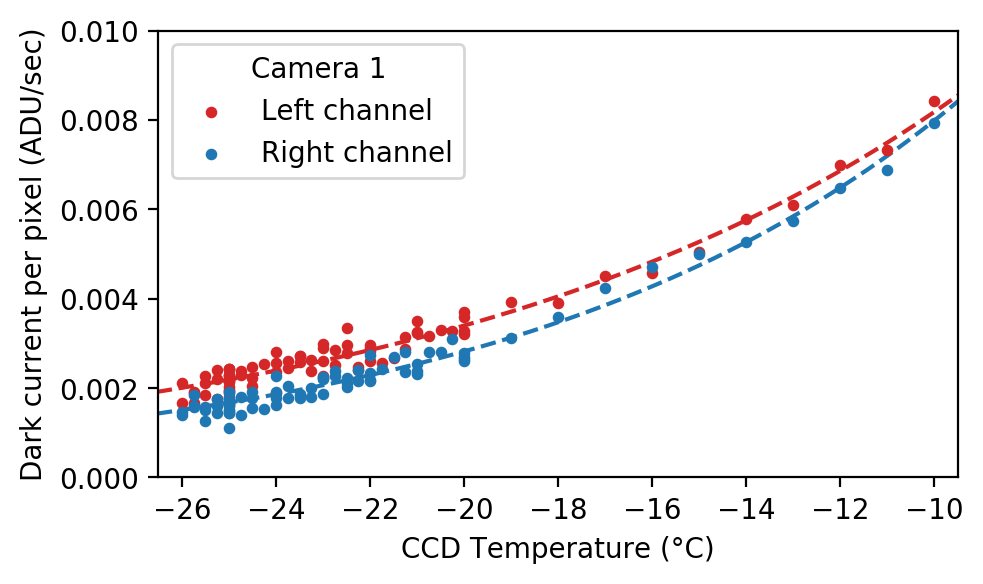
\includegraphics[width=\linewidth]{images/detectors/dc_1.png}
        \end{minipage}
        \begin{minipage}[t]{0.49\textwidth}\vspace{10pt}
            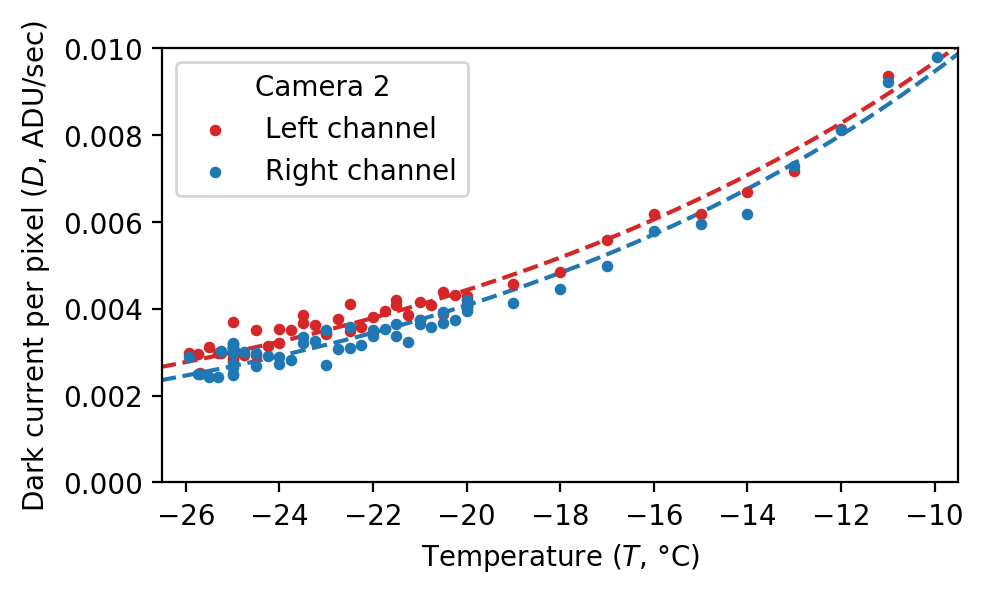
\includegraphics[width=\linewidth]{images/detectors/dc_2.png}
        \end{minipage}

        \begin{minipage}[t]{0.49\textwidth}\vspace{10pt}
            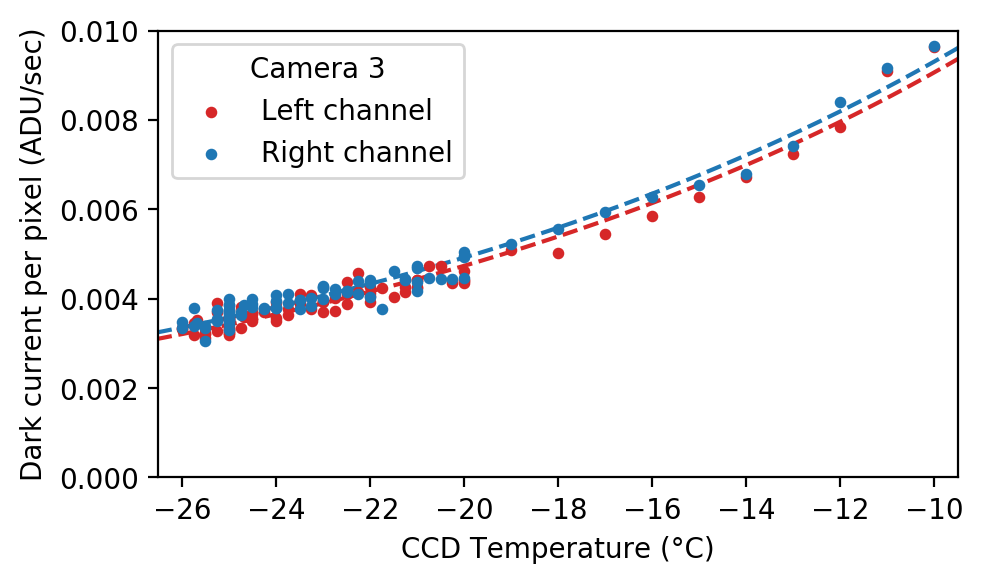
\includegraphics[width=\linewidth]{images/detectors/dc_3.png}
        \end{minipage}
        \begin{minipage}[t]{0.49\textwidth}\vspace{10pt}
            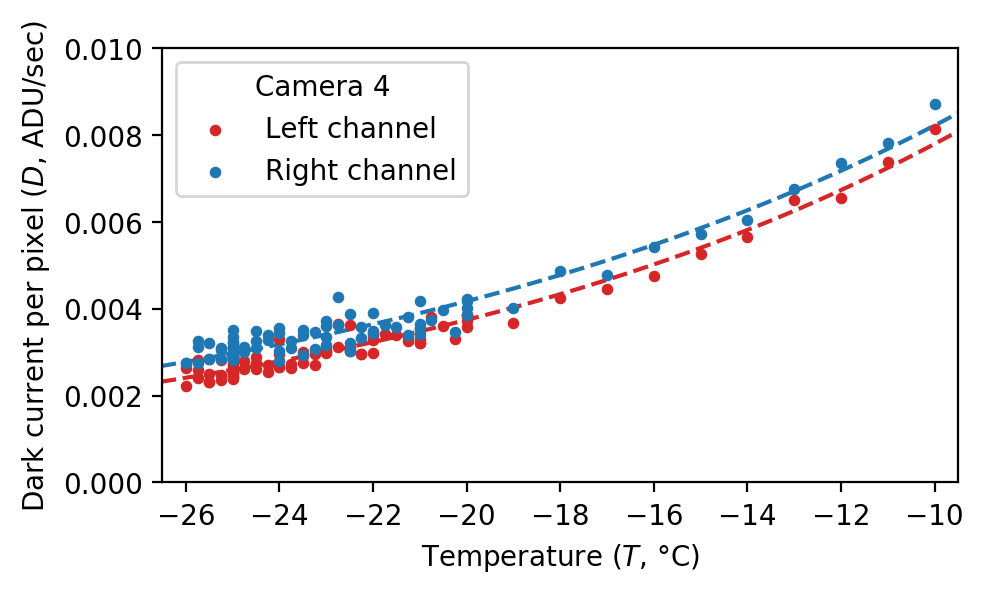
\includegraphics[width=\linewidth]{images/detectors/dc_4.png}
        \end{minipage}

        \begin{minipage}[t]{0.49\textwidth}\vspace{10pt}
            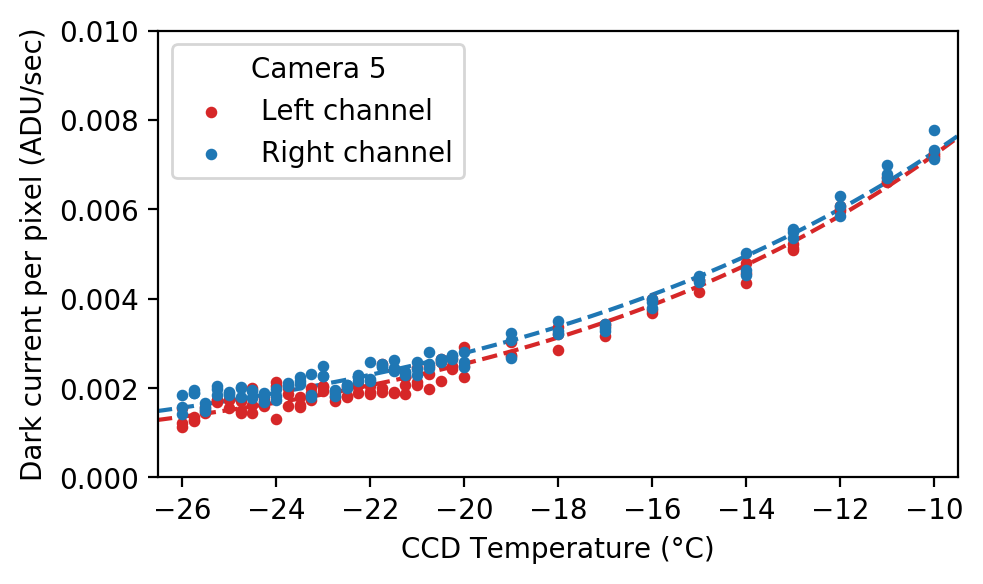
\includegraphics[width=\linewidth]{images/detectors/dc_5.png}
        \end{minipage}
        \begin{minipage}[t]{0.49\textwidth}\vspace{10pt}
            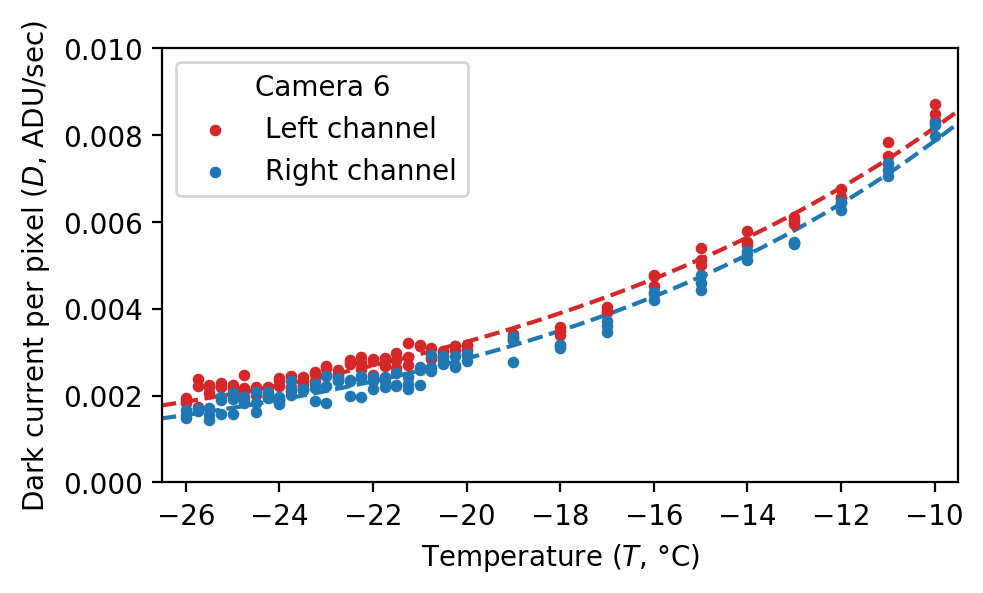
\includegraphics[width=\linewidth]{images/detectors/dc_6.png}
        \end{minipage}

        \begin{minipage}[t]{0.49\textwidth}\vspace{10pt}
            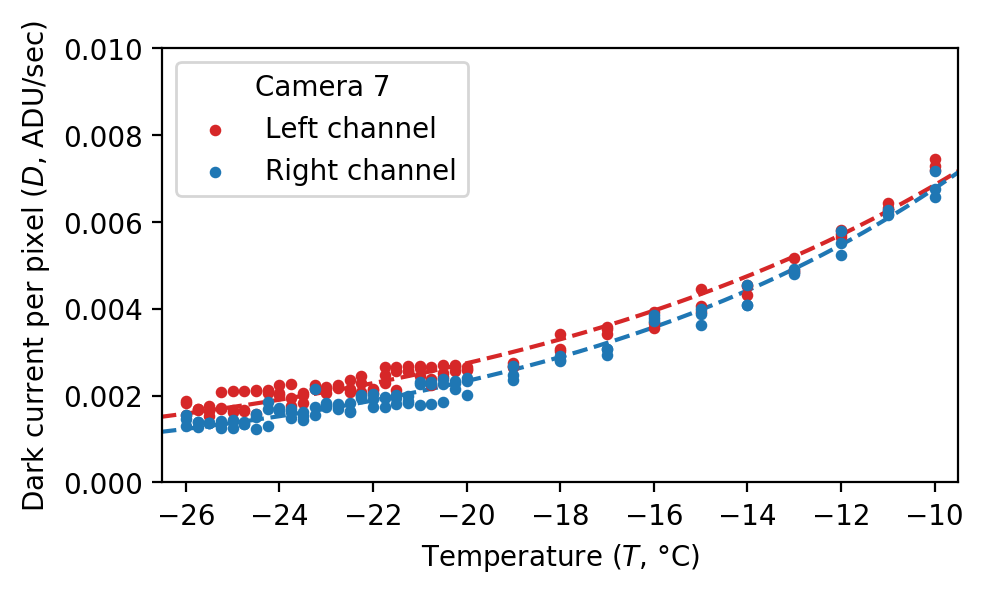
\includegraphics[width=\linewidth]{images/detectors/dc_7.png}
        \end{minipage}
        \begin{minipage}[t]{0.49\textwidth}\vspace{10pt}
            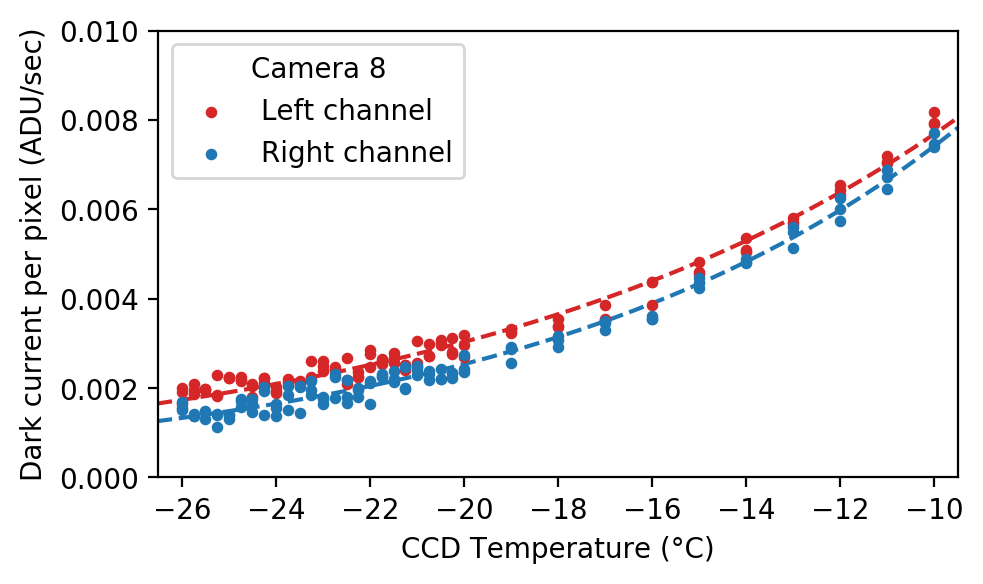
\includegraphics[width=\linewidth]{images/detectors/dc_8.png}
        \end{minipage}
    \end{center}
    \caption[Dark current plots]{
        Dark current plots for each camera.
    }\label{fig:dcs}
\end{figure}

\clearpage

\end{colsection}

% ~~~~~~~~~~~~~~~~~~~~
\newpage
\subsection{Linearity}
\label{sec:lin}
\begin{colsection}

Linearity is a measure of the response of the CCD over its entire dynamic range. The output count should always be linearly related to the input photons, and for scientific imaging it is particularly important that the measured counts are directly proportional to the object signal.

The non-linearity of each camera was measured using the same images taken for the photon transfer curves in \aref{sec:ptc}, bright images of a flat source with increasing exposure times. The images were bias-subtracted, and the mean counts of a central 2000$\times$2000 pixel region in the centre of each channel was plotted against the exposure time, shown in \aref{fig:lin}. A linear relation was fitted to the central potion of the data, excluding the upper and lower 10\% of the dynamic range. Residuals from this fit as a percentage of the count are also plotted in \aref{fig:lin}, and the mean absolute deviation from the linear fit over the central region is given in \aref{tab:lin}.

The values for non-linearity measured vary greatly between each camera, and several are over 1\%. If these values were true this would be a major problem when making accurate photometric measurements. However, the FLI specification advertises a non-linearity of <1\%, and FLI's own tests of the cameras consistently report non-linearity of 0.2\% or less. Accurately measuring the response of a CCD requires a perfectly uniform light source and an integrating sphere, which FLI would have access to. I had to make do with a LCD screen when carrying out the tests in the lab, which is a poor substitute. Therefore the values in \aref{tab:lin} should not be considered reliable measurements.

\begin{table}[t]
    \begin{center}
        \begin{tabular}{c|cc} %chktex 44
             & \multicolumn{2}{c}{Non-linearity} \\
             & \multicolumn{2}{c}{(\%)} \\
             & \multicolumn{1}{c}{L} & \multicolumn{1}{c}{R} \\
            \midrule
            Camera 1 & 2.29 & 2.00 \\
            Camera 2 & 0.76 & 0.65 \\
            Camera 3 & 0.34 & 0.39 \\
            Camera 4 & 0.18 & 0.22 \\
        \end{tabular}
        \hspace{0.5cm}
        \begin{tabular}{c|cc} %chktex 44
             & \multicolumn{2}{c}{Non-linearity} \\
             & \multicolumn{2}{c}{(\%)} \\
             & \multicolumn{1}{c}{L} & \multicolumn{1}{c}{R} \\
            \midrule
            Camera 5 & 1.25 & 1.20 \\
            Camera 6 & 1.20 & 1.13 \\
            Camera 7 & 0.70 & 0.68 \\
            Camera 8 & 0.82 & 0.80 \\
        \end{tabular}
    \end{center}
    \caption[Non-linearity values]{
        Non-linearity values for each camera.
    }\label{tab:lin}
\end{table}

\begin{figure}[p]
    \begin{center}
        \begin{minipage}[t]{0.49\textwidth}\vspace{10pt}
            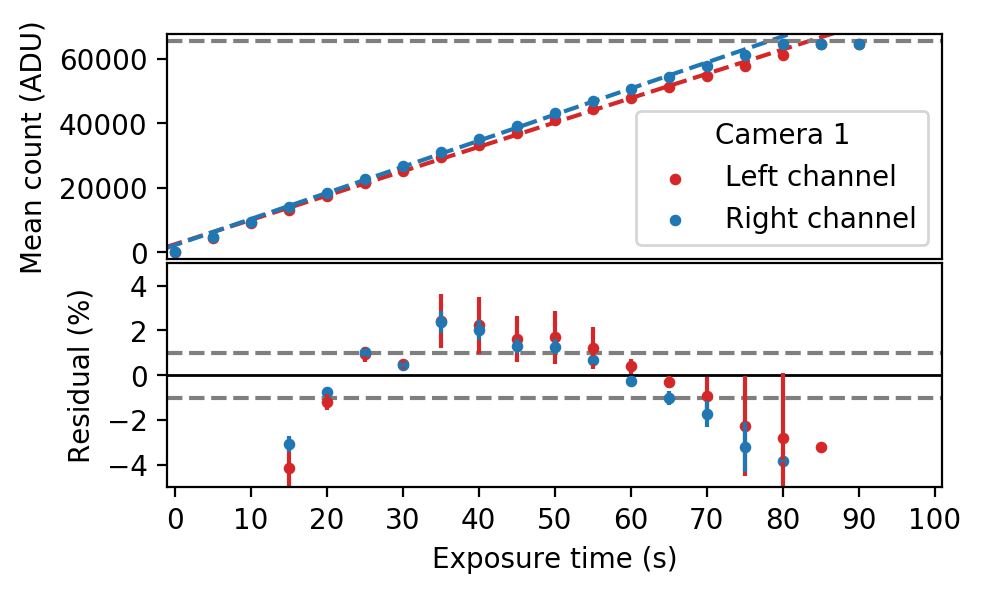
\includegraphics[width=\linewidth]{images/detectors/lin_1.png}
        \end{minipage}
        \begin{minipage}[t]{0.49\textwidth}\vspace{10pt}
            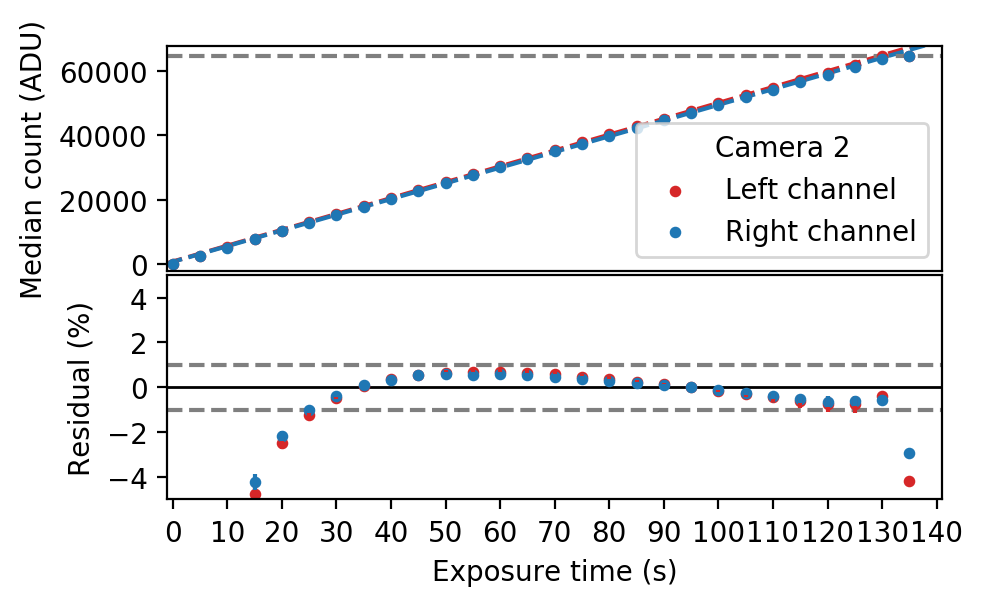
\includegraphics[width=\linewidth]{images/detectors/lin_2.png}
        \end{minipage}

        \begin{minipage}[t]{0.49\textwidth}\vspace{10pt}
            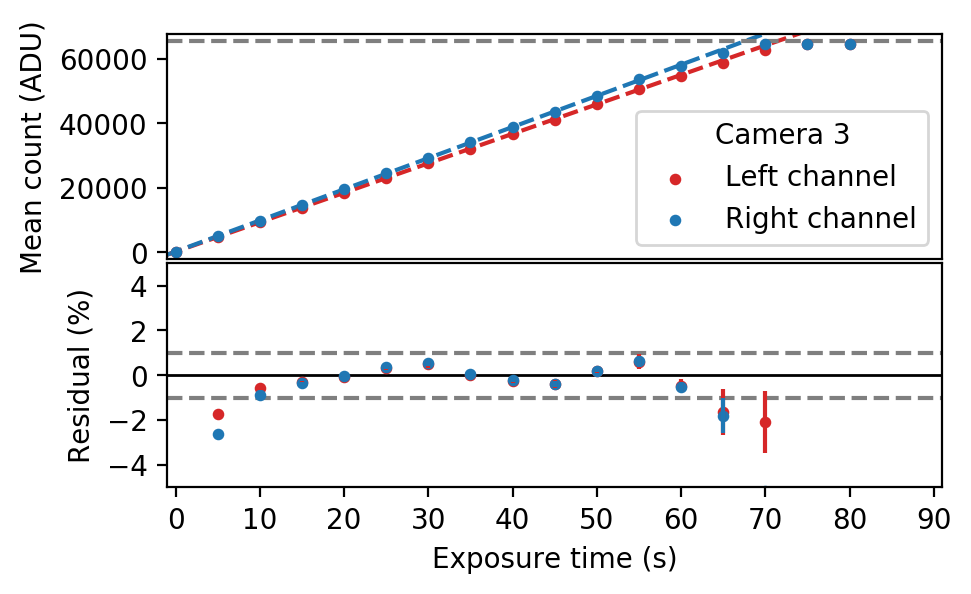
\includegraphics[width=\linewidth]{images/detectors/lin_3.png}
        \end{minipage}
        \begin{minipage}[t]{0.49\textwidth}\vspace{10pt}
            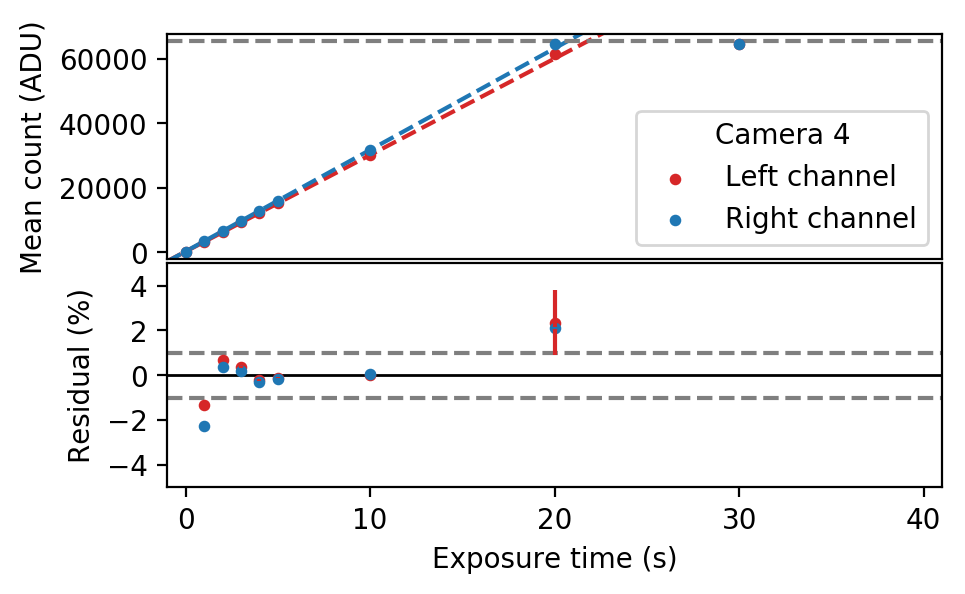
\includegraphics[width=\linewidth]{images/detectors/lin_4.png}
        \end{minipage}

        \begin{minipage}[t]{0.49\textwidth}\vspace{10pt}
            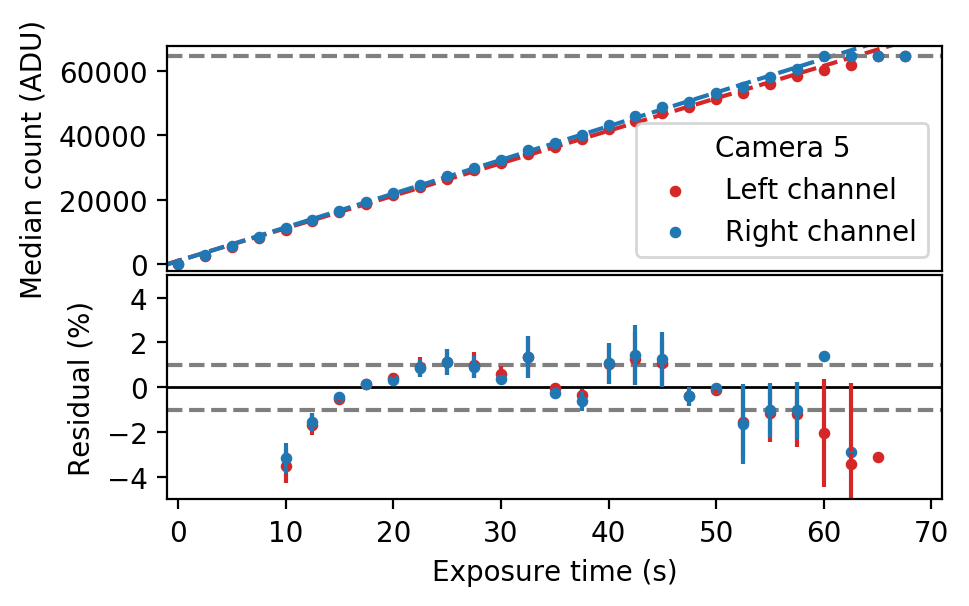
\includegraphics[width=\linewidth]{images/detectors/lin_5.png}
        \end{minipage}
        \begin{minipage}[t]{0.49\textwidth}\vspace{10pt}
            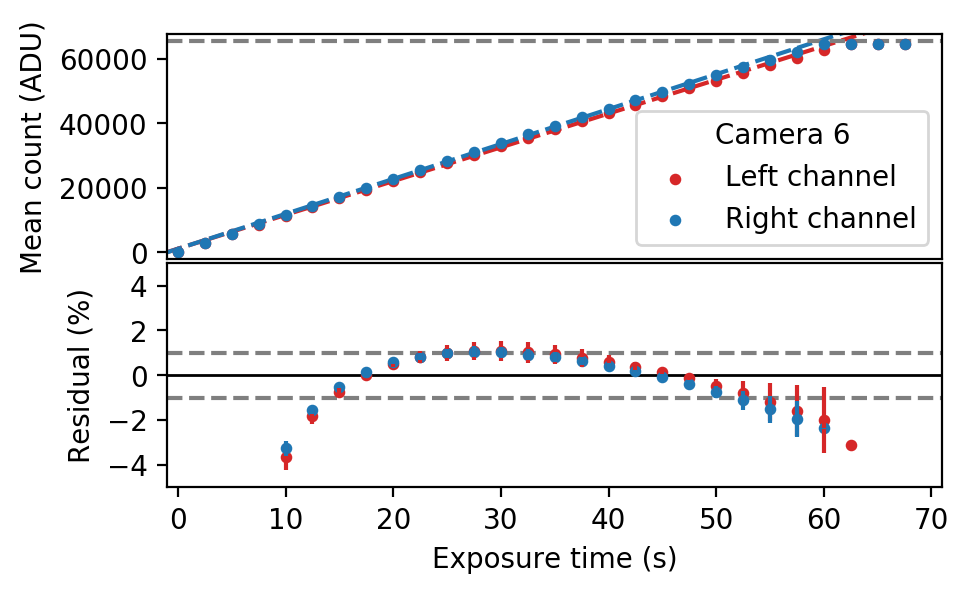
\includegraphics[width=\linewidth]{images/detectors/lin_6.png}
        \end{minipage}

        \begin{minipage}[t]{0.49\textwidth}\vspace{10pt}
            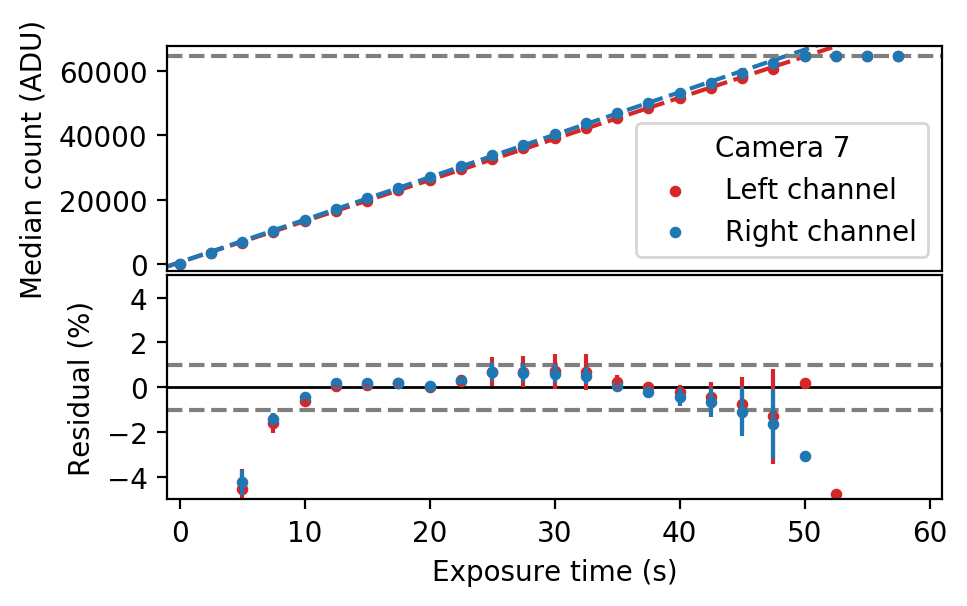
\includegraphics[width=\linewidth]{images/detectors/lin_7.png}
        \end{minipage}
        \begin{minipage}[t]{0.49\textwidth}\vspace{10pt}
            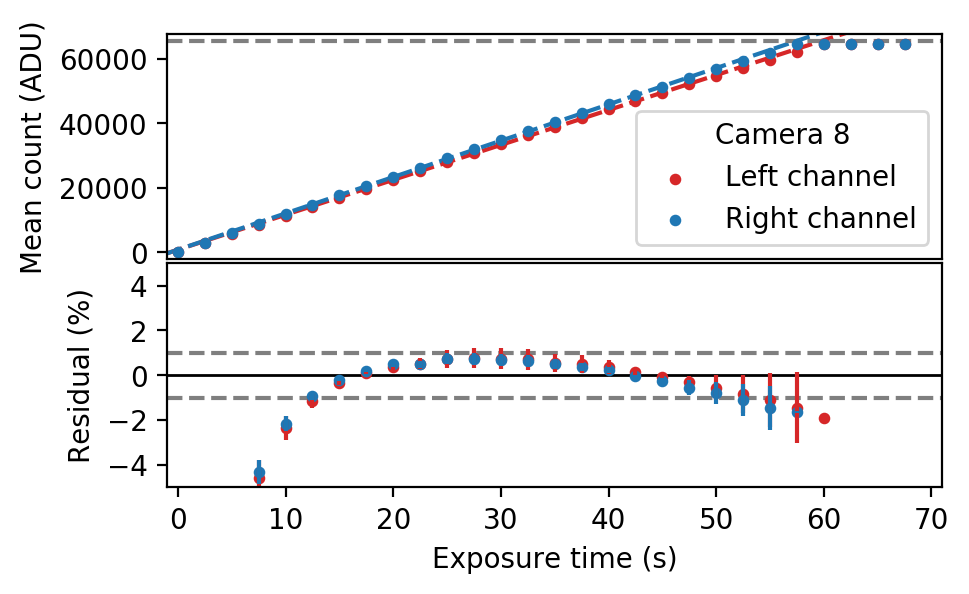
\includegraphics[width=\linewidth]{images/detectors/lin_8.png}
        \end{minipage}
    \end{center}
    \caption[Linearity plots]{
        Linearity plots for each camera.
    }\label{fig:lin}
\end{figure}

\clearpage

\end{colsection}

% ~~~~~~~~~~~~~~~~~~~~
\newpage
\subsection{Defects}
\label{sec:defects}
\begin{colsection}

There are several possible defects in CCD sensors \citep{CCDs}: hot pixels, which have atypically high dark currents, dead pixels, which produce zero counts, and trap pixels, which ``trap'' electrons and prevent read out from it and any pixels above it in the column. For targeted astronomical observations it is important to track any bad pixels, so whenever possible photons from the target object does not fall on any of them. GOTO's wide-field survey observations make this less of an issue, but the pipeline will track bad pixels and columns when calibrating images from each camera.

Single hot or dead pixels are not a major problem, as they can be removed by subtracting bias frames and flat fielding. If necessary the value of the bad pixel can be interpolated from the surrounding pixels. Trap pixels are more of an issue, as they take out the entire column behind them. For each camera a defect mask was made by taking the ratio of two flat images with different exposure times, making any bad pixels or columns easy to pick out by comparing to the surrounding pixels. And example of a trap pixel is shown in \aref{fig:itsatrap}. The positions of trap pixels for each camera are given in \aref{tab:traps}. The KAF-50100 chip specification gives an allowed limit of less than 20 column defects per device, which the GOTO cameras are well within.

\begin{table}[t]
    \begin{center}
        \begin{tabular}{c|ccc} %chktex 44
             & \multicolumn{2}{c}{Trap location} & Column lost \\
             & x & y & \% \\
            \midrule
            Camera 1 & 7751 & 4361 & 30 \\
            Camera 2 & 1658 & ~172 & 97 \\ %chktex 39
            Camera 3 & 1224 & 1844 & 70 \\
                     & 5058 & 5185 & 17 \\
            Camera 4 & 5406 & 2607 & 58 \\
            Camera 5 & 6293 & 1416 & 77 \\
            Camera 6 & 5455 & 5036 & 19 \\
        \end{tabular}
        \hspace{0.5cm}
        \begin{tabular}{c|ccc} %chktex 44
            & \multicolumn{2}{c}{Trap location} & Column lost \\
            & x & y & \% \\
            \midrule
            Camera 7 & 1344 & 3037 & 51 \\
                     & 2326 & 2495 & 60 \\
                     & 2610 & 5688 & ~9 \\ %chktex 39
                     & 7491 & 5120 & 18 \\
            Camera 8 & 1184 & 3043 & 51 \\
                     & 5659 & 2778 & 55 \\
            \multicolumn{4}{c}{} \\
        \end{tabular}
    \end{center}
    \caption[Locations of trap pixels]{
        Locations of trap pixels and fraction of the column lost for each camera.
    }\label{tab:traps}
\end{table}

\begin{figure}[p]
    \begin{center}
        \includegraphics[width=\textwidth]{images/detectors/defect_plot.pdf}
    \end{center}
    \caption[An example of a trap pixel]{
        A flat frame for Camera 1 showing an example of a trap pixel. The plot below of counts averaged in the y axis clearly shows the bad column, and the depth of the well beneath the field level is proportional to the height of the trap pixel in the column.
    }\label{fig:itsatrap}
\end{figure}

\clearpage

\end{colsection}

% ~~~~~~~~~~~~~~~~~~~~

\end{colsection}

% ########################################

\newpage
\section{System throughput}
\label{sec:throughput}
\begin{colsection}

% ~~~~~~~~~~~~~~~~~~~~

\begin{colsection}

The throughput is important to measure.

It's made up of a variety of elements.

\end{colsection}

% ~~~~~~~~~~~~~~~~~~~~
\subsection{Optical elements}
\label{sec:optics}
\begin{colsection}

The GOTO unit telescopes are Wynne-Newtonian astrographs manufactured by APM Telescopes\footnote{\url{https://www.professional-telescopes.com/}}. They are fast Newtonian telescopes with a \SI{40}{\centi\meter} primary mirror and a flat \SI{19}{\milli\meter} (on the short axis) elliptical secondary. Between the secondary and the camera is a three-lens Wynne corrector to focus the light back onto the CCD detector. The full \gls{ota} design is shown in \aref{fig:ota}, and the five elements the light must pass through (the three corrector lenses, the filter in the filter wheel and the window in front of the detector) are shown in \aref{fig:wynne}.


\begin{figure}[p]
    \begin{center}
        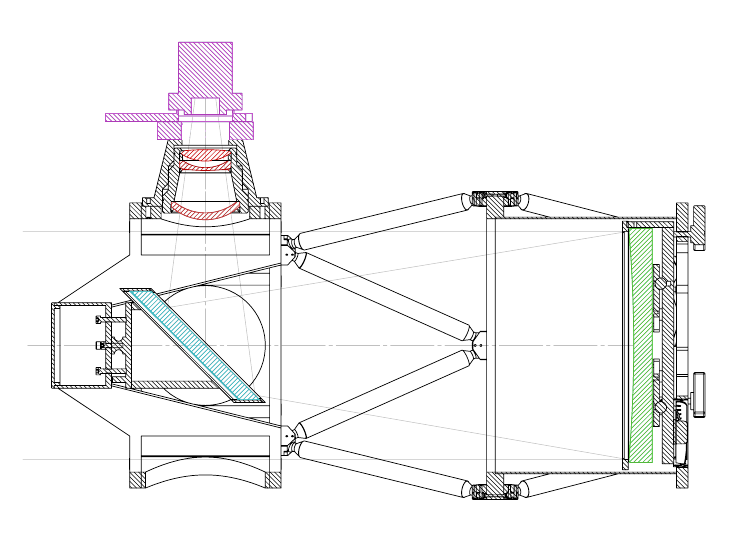
\includegraphics[width=0.7\textwidth]{images/throughput/OTA_optics.png}
    \end{center}
    \caption[GOTO optical telescope assembly]{
        The \gls{ota} design for one of the GOTO prototype unit telescopes. Light enters from the left, and the optical elements have been highlighted: the primary mirror in \textcolor{Green}{\textbf{green}}, the secondary mirror in \textcolor{BlueGreen}{\textbf{blue}}, the Wynne corrector lenses in \textcolor{Red}{\textbf{red}} and the FLI camera hardware (focuser, filter wheel and camera) in \textcolor{Purple}{\textbf{purple}}.
    }\label{fig:ota}
\end{figure}

\begin{figure}[p]
    \begin{center}
        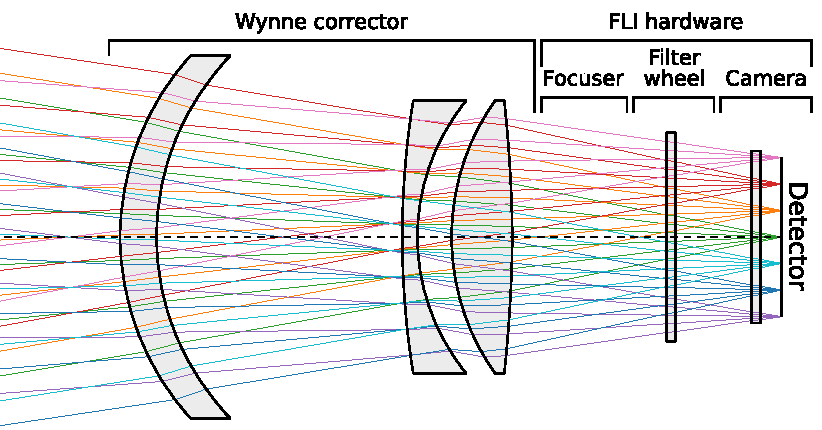
\includegraphics[width=0.7\textwidth]{images/throughput/wynne.pdf}
    \end{center}
    \caption[Ray tracing the corrector elements]{
        A ray trace showing the optical elements after the secondary mirror. From left-to-right light passes through the three corrector lenses, the filter and the camera window before reaching the detector located in the focal plane.
    }\label{fig:wynne}
\end{figure}

\clearpage

\end{colsection}

% ~~~~~~~~~~~~~~~~~~~~
\newpage
\subsection{Colour filters}
\label{sec:filters}
\begin{colsection}

\rtxt{TODO}

\end{colsection}

% ~~~~~~~~~~~~~~~~~~~~
\newpage
\subsection{Atmospheric extinction}
\label{sec:atmosphere}
\begin{colsection}

\rtxt{TODO}

\end{colsection}

% ~~~~~~~~~~~~~~~~~~~~
\newpage
\subsection{Throughput modelling}
\label{sec:synphot}
\begin{colsection}

\rtxt{TODO}

\end{colsection}

% ~~~~~~~~~~~~~~~~~~~~
\newpage
\subsection{Comparison to on-sky zeropoints}
\label{sec:onsky_throughput}
\begin{colsection}

\rtxt{TODO}

\end{colsection}

% ~~~~~~~~~~~~~~~~~~~~

\newpage
\subsection{Predicting exposure times}
\label{sec:etc}
\begin{colsection}

\rtxt{TODO}

\end{colsection}

% ~~~~~~~~~~~~~~~~~~~~

\end{colsection}

% ########################################
